\subsection{History Retention and Transfer Across Plants}
\label{sec:c03}
The controlled comparison separates retaining recovery histories (history)
from merging restored histories into the augmented state mean (carry), with nominal
conditional covariance shared, and from resetting that state (reset). All
arms use the frozen admission, reporting, severity, and instrumental-state
rules. The primary endpoint is correct family and source attribution before
restoration. Event-record extras are distinct from normal-operation alarms.

In F01, history attributed \CThreeFOneHistoryShortTimely{} of
\CThreeAuditFZeroOneHistoryShortN{} primary interventions in time, versus
\CThreeFOneCarryShortTimely{} for carry and \CThreeFOneResetShortTimely{}
for reset. The paired history-minus-carry coverage difference was
\CThreeFOneHistoryCarryDifferencePP{} percentage points (95\% interval
\CThreeFOneHistoryCarryLowerPP{}--\CThreeFOneHistoryCarryUpperPP{});
the difference in event-record extras was
\CThreeFOneHistoryCarryExtraRateDiff{} per monitored event-hour (95\% interval
\CThreeFOneHistoryCarryExtraRateLower{}--\CThreeFOneHistoryCarryExtraRateUpper{}).
In P2, history and carry attributed \CThreePTwoHistoryShortTimely{} and
\CThreePTwoCarryShortTimely{} of \CThreeAuditPTwoHistoryShortN{} primary
interventions, respectively. Their paired difference was
\CThreePTwoHistoryCarryDifferencePP{} points (95\% interval
\CThreePTwoHistoryCarryLowerPP{}--\CThreePTwoHistoryCarryUpperPP{}), which
does not establish a coverage gain. The extra-rate difference was
\CThreePTwoHistoryCarryExtraRateDiff{} per event-hour (95\%
interval \CThreePTwoHistoryCarryExtraRateLower{}--
\CThreePTwoHistoryCarryExtraRateUpper{}). Thus the comparison supports a history
advantage over carry in F01, but not a transferred coverage advantage in
P2. In both plants, carry substantially outperformed reset on coverage and
event extras, supporting continuity of the estimated physical state. This
result does not isolate semantic history labels from every other aspect of
the procedure.

All arms passed CAL feasibility. CAL selected thresholds
\CThreeCalHistoryThreshold{} (history and carry) and
\CThreeCalResetThreshold{} (reset), with zero alarms over
\CThreeFOneHistoryNormalHours{} normal hours per arm. TEST also had zero
normal alarms in \CThreeFOneHistoryNormalHours{} hours per arm (one-sided
95\% Poisson upper bound \CThreeFOneHistoryNormalUpper{}/h). This exposure
does not verify a long-run 1/h guarantee. Under dropout stress, nominal
calibration was not repeated: normal alarms were \CThreeAuditFZeroOneDropoutNormalAlarms{} in \CThreeAuditFZeroOneDropoutNormalHours{} h for F01 (upper bound \CThreeAuditFZeroOneDropoutNormalUpper{}/h) and \CThreeAuditPTwoDropoutNormalAlarms{} in \CThreeAuditPTwoDropoutNormalHours{} h for P2 (upper bound \CThreeAuditPTwoDropoutNormalUpper{}/h). The independent-noise stress
cohort was unavailable for \CThreeAuditFZeroOneNoiseUnavailable{} of \CThreeAuditFZeroOneNoiseParents{} F01 parents and \CThreeAuditPTwoNoiseUnavailable{} of \CThreeAuditPTwoNoiseParents{} P2 parents because the
prefix noise estimate exceeded its frozen support; it provides no
performance estimate.

Figure~\ref{fig:c03} summarizes primary coverage, event-record extras, and
the paired history-minus-carry coverage contrast. The result is conditional
on the two tested simulator configurations and frozen sequential protocol;
it does not establish transfer to other plant families.

\begin{figure*}[t]
\centering
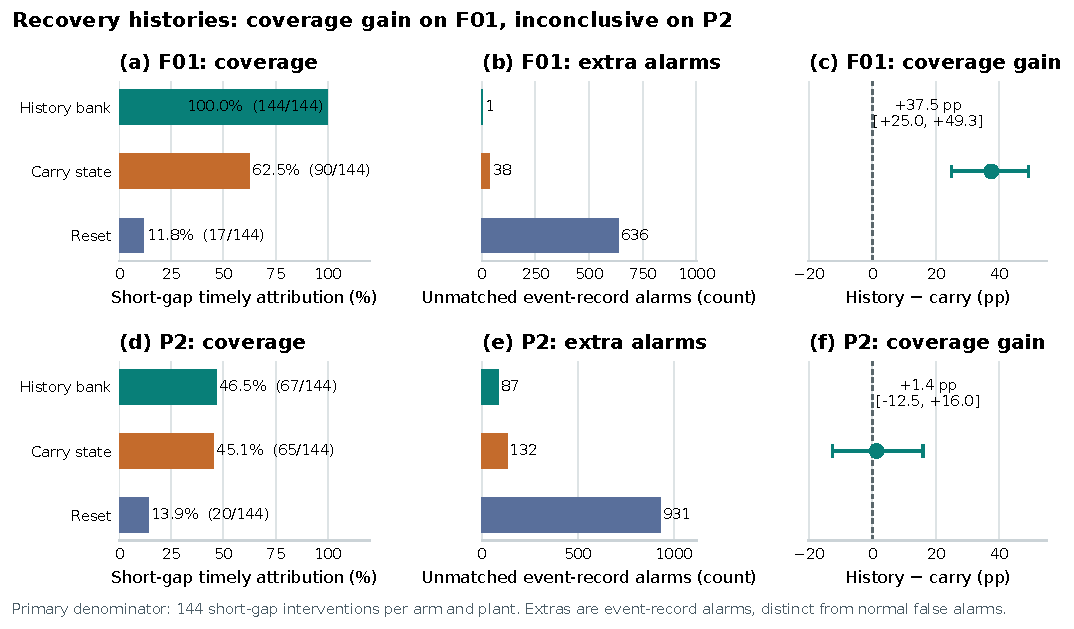
\includegraphics[width=.98\textwidth]{figures/generated/recovery_c03.pdf}
\caption{C03 held-out results from the sealed evaluation. Timely coverage
uses the primary short-gap interventions per arm and plant. Event-record
extras are unmatched alarms during event records, distinct from normal
false alarms. The paired history-minus-carry contrast favors history in F01;
the interval includes zero in P2. Reset has lower coverage and many more
extras than carry in both plants.}
\label{fig:c03}
\end{figure*}
